\documentclass[12pt]{article}
\usepackage{float}
\usepackage{graphicx}
\usepackage[fleqn]{amsmath}
\usepackage{amssymb}
\usepackage{parskip}
\usepackage[a4paper,top=2cm,bottom=2cm,left=3cm,right=3cm,marginparwidth=1.75cm]{geometry}

% \setlength{\parindent}{0pt}

\begin{document}

\date{}
\author{Marco Sterlini}

\title{Notes on Event-triggered neural network control using quadratic constraints for perturbed systems paper}

\maketitle

From \textbf{Event-triggered neural network control using quadratic constraints for perturbed systems} paper it is useful to extract the application of the ETM mechanism directly inside the NN controller to decide whether to propagate an input. 
With respect to CSS paper there's a generalization of the activation function, no more restricted to saturation only and the structure of the ETM, error based in CSS and QC based here. Also, the system here is perturbed.

The plant to control is represented with $\mathbb{G}(G, \Delta)$ meaning the linear part $G$ and the non-linear perturbation part $\Delta$. It is described by:

\begin{equation}
  \begin{aligned}
    x(k+1) &= A_G x(k) + B_{G_u} u(k) + B_{G_q} q(k), \\
    p(k) &= C_G x(K) + D_{G_u} u(k) + B_{G_q} q(k),
  \end{aligned}
\end{equation}

With $p$ and $q$ being the input and output of the perturbation block $\Delta$: $q(\cdot) = \Delta(p(\cdot))$

\begin{figure}[H]
    \centering
    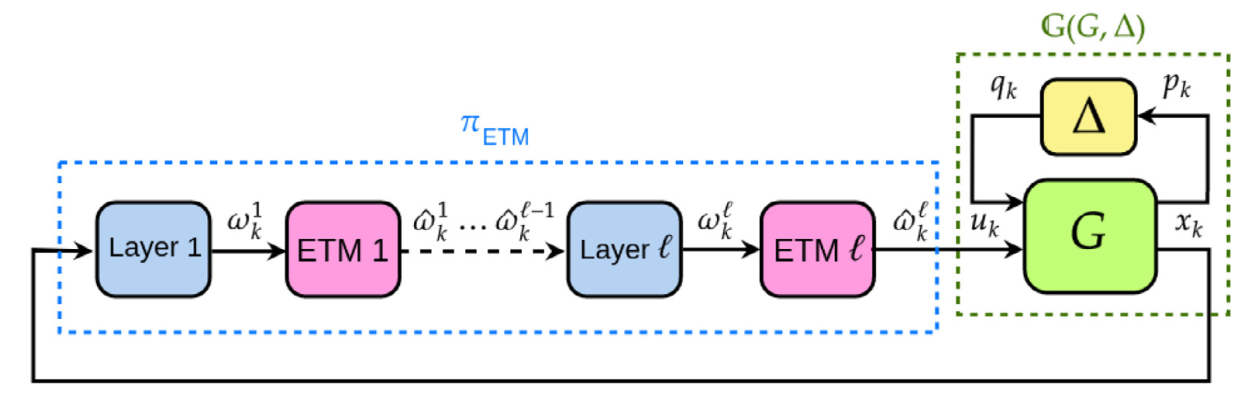
\includegraphics[width=0.65\textwidth]{img/scheme.png}
    \caption{Overall scheme of the controlled plant}
    \label{}
\end{figure}

\textbf{Notation on controller $\pi_{ETM}$}

The controller is a Feed Forward Neural Network of $l$ layers. With $\hat{w}$ it is intended the last transmitted output of a layer, with $\omega$ the current output of the layer and with $\nu$ the input to the activation function.

\begin{equation}
  \begin{aligned}
    \hat{\omega}^0(k) &= x(k), \\    
    \nu^i(k) &= W^i \hat{\omega}^{i-1}(k) + b^i, \\
    \omega^i(k) &= \phi^i( \nu^i(k)), \\
    u(k) &= W^{l+1} \hat{\omega}^l(k) + b^{l+1},
  \end{aligned}
\end{equation}

Where the input signal $u(k)$ is the output of the last layer and $b^i$ represents the bias vector of the $i^{th}$ layer.
Everything is vectorized so to isolate the non-linearities:

\begin{equation}
  \begin{bmatrix}
    u(k)\\
    \nu_{\phi}(k)
  \end{bmatrix} = N \begin{bmatrix}
    x(k)\\
    \hat{\omega}(k)\\
    1
  \end{bmatrix}
\end{equation}

Where $N$ is the matrix like in equation 8 of the paper.

Then follows the modelling of the perturbations, I won't treat it for now. Just to sum it up the perturbation block is modelled as a filter (equation. 9 and 10 in the paper) and the output of this filter $r(k)$ respects an Integral (a sum in DT) Quadratic Constraint, this means that the perturbation $\Delta$ must satisfy a specific energy-like inequality over time.

Then it is introduced the \textit{Local Sector Condition} used to deal with non-linear functions in a given interval. This will be used to treat the activation functions close the equilibrium. The non-linear function will be encapsulated in linear bounds that will then be directly injected in the stability LMI conditions.

Lemma 1 introduces a way to express the local sector condition for non-linearity $\phi$ in a compact form using the matrix $\Pi_{ds}$ called \textit{Diagonally structured multiplier} that belongs to a class of polytopic bounding multipliers, then another lemma is introduced for the latter. 

After the applications of all these lemmas, equation 19 is obtained. 

It is then defined the new ETM policy, that doesn't rely on the error like in the previous paper, the quadratic constraint instead measures the deviation of the pair $(\nu, \omega)$ from the equilibrium one, it represents if the system is behaving as expected or not and hence if it requires an update. 

\begin{equation}
  \hat{\omega}^i(k) = \begin{cases}
    \hat{\omega}(k-1), & \text{if } [\bullet ]^{\top} \Pi_i \begin{bmatrix}
      \nu^i(k) - \nu_*^i \\
      \hat{\omega}^i(k-1) - \omega_*^i
    \end{bmatrix} \geq 0.\\
    \omega^i(k), & \text{otherwise}
  \end{cases}
\end{equation}

For all $i=1, \dots, l$.

Like in the previous paper it holds that if a layer is not updated all the following ones won't be also. 

In the rest of the paper it was treated the problem of designing the triggering parameters that characterize $\Pi$ while assuring the stable behavior of the system. An augmented state vector that takes into account the perturbation has been used and in order to design the ETM matrix Theorem 1 has been stated and proved. Everything so that equation 26, the LMI condition for Lyapunov stability, holds. Adding another condition the LMI solution would give as a result also an estimate of the region of attraction, the problem is that this system is composed of infinite equations, to address this problem adding a constraint in $\Pi$ the number becomes finite. An optimization problem than has been developed to maximize the trade-off between size of the region of attraction and the saving in computation of the neural network.

Simulations were run for different values for both $\alpha$ and $\beta$ to better show how the performance change along the trade-off. It has been shown that for 4 layers architectures the computational saving can add up to 50\%.
\end{document}

% \begin{figure}[H]
%     \centering
%     \begin{subfigure}{0.4\textwidth}
%     \includegraphics[width=\textwidth]{}
%     \caption{}
%     \label{}
%     \end{subfigure}
%     \hfill
%     \begin{subfigure}{0.55\textwidth}
%     \includegraphics[width=\textwidth]{}
%     \caption{}
%     \label{}
%     \end{subfigure}
%     \caption{}
%     \label{}
% \end{figure}

% \begin{figure}[H]
%     \centering
%     \includegraphics[width=0.65\textwidth]{}
%     \caption{}
%     \label{}
% \end{figure}